\documentclass[10pt]{beamer}
\usetheme{Luebeck}
\usepackage[utf8]{inputenc}
\usepackage{amsmath}
\usepackage{amsfonts}
\usepackage{amssymb}
\usepackage{graphicx}
\newcommand\tab[1][0.5cm]{\hspace*{#1}}

\author{Galal, Mido, Mona, Omar}

\title{%
		Computer Vision Course Project \\
  \small Face Detection with Python}

%\setbeamercovered{transparent} 
%\setbeamertemplate{navigation symbols}{} 
%\logo{} 
%\institute{} 
%\date{} 
%\subject{} 
\begin{document}


\begin{frame}
\titlepage
\end{frame}


\begin{frame}
\tableofcontents
\end{frame}

\section{Problem Definition and Motivation}

\subsection{Problem Definition}

\begin{frame}{Problem Definition and Motivation}

\begin{figure}
\vspace*{-1cm}
\hspace*{8.2cm}
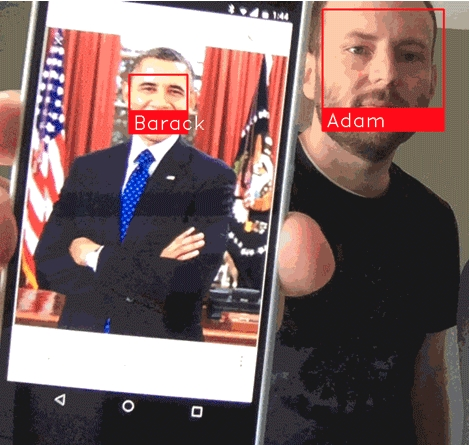
\includegraphics[scale=0.2]{images/obama}
\end{figure}

\vspace*{-5cm}
\hspace*{0cm}

Face detection is a computer technology being used \\
in a variety of applications that identifies human \\
faces in digital images.\\~\\


The basic benefit of the technology is to detect human \\
faces, regardless of identity of the person. \\
But a more advanced version of it, coupled with \\
maching learning and training on pre-acquired images, \\
it can detect a person's face and who really is him.

\end{frame}


\subsection{Motivation}
\begin{frame}{Problem Definition and Motivation}

\begin{figure}
\vspace*{0cm}
\hspace*{0cm}
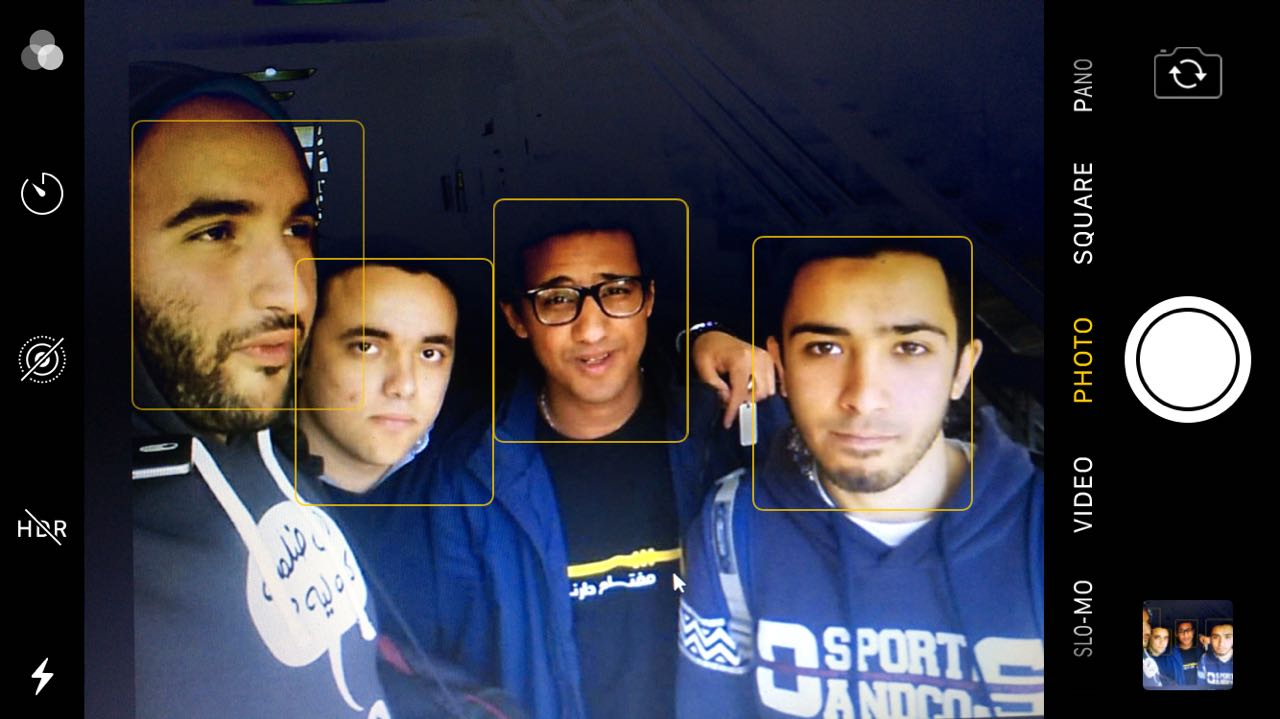
\includegraphics[scale=0.15]{images/camera}
\end{figure}

We deal with face detection in our daily life. One simple example is when you're trying to photograph your friends and then your phone camera detects faces and put green rectangles around them.
\end{frame}


\begin{frame}{Problem Definition and Motivation}

\begin{figure}
\vspace*{0cm}
\hspace*{0cm}
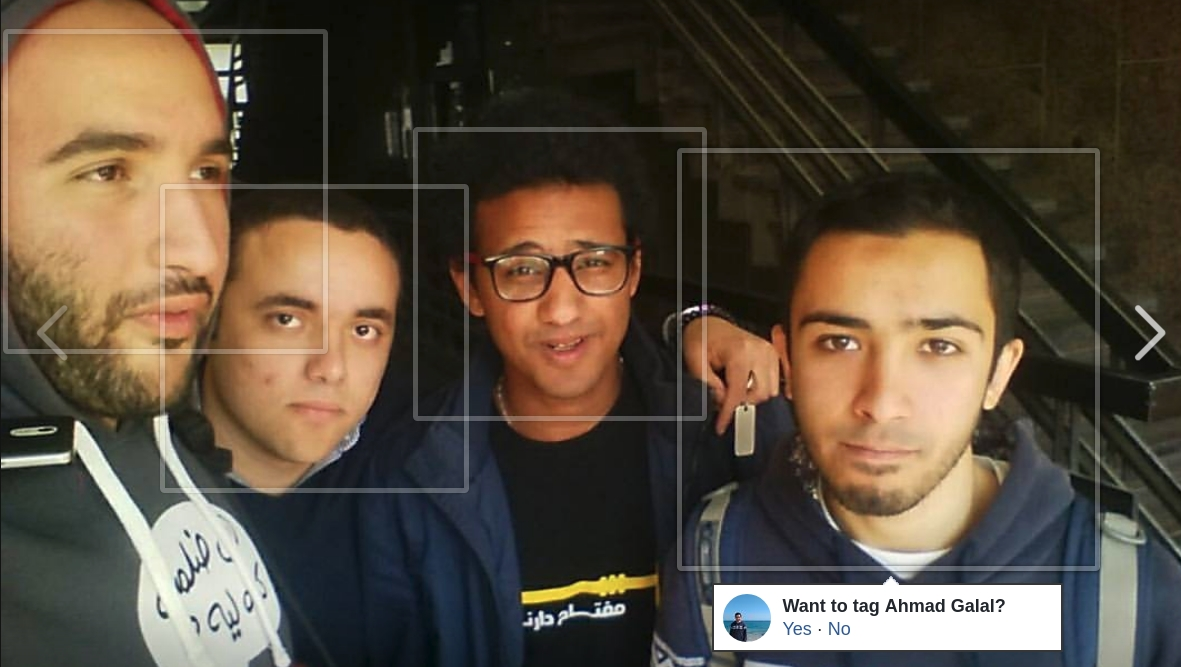
\includegraphics[scale=0.15]{images/modMen}
\end{figure}

Another more common example is when you upload the photo you just captured in the previous slide to Facebook, and you find it putting the same rectangles around each face \textbf{plus} suggesting a tag for each one.
\end{frame}






\section{Algorithms Used}
\begin{frame}{Algorithms Used}

\textbf{Goal:} \\
\tab Using Haar Cascade Classifiers to detect faces, eyes, smiles, ...etc \\~\\~\\

\textbf{Intro:} \\
\tab Object Detection using Haar feature-based cascade classifiers is an effective object detection method proposed by Paul Viola and Michael Jones in 2001. It is a machine learning based approach where a cascade function is trained from a lot of positive and negative images. It is then used to detect objects in other images.
\end{frame}


\begin{frame}{Algorithms Used}


\textbf{How it works in the background:} \\
\tab Now we need to extract features from the training images. For this, Haar features shown in the below image are used. They are just like our convolutional kernel. Each feature is a single value obtained by subtracting sum of pixels under the white rectangle from sum of pixels under the black rectangle. \\~\\

All possible sizes and locations of each kernel are used to calculate lots of features. For each feature calculation, we need to find the sum of the pixels under white and black rectangles.

\begin{figure}
\vspace*{0cm}
\hspace*{0cm}
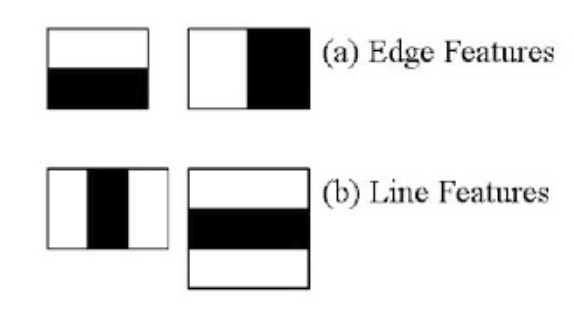
\includegraphics[scale=0.25]{images/kernel}
\end{figure}
\end{frame}



\begin{frame}{Algorithms Used}
We apply each and every feature on all the training images. For each feature, it finds the best threshold which will classify the faces to positive and negative. We select the features that most accurately classify the face and non-face images. \\~\\

The final classifier is a weighted sum of these weak classifiers. It is called weak because it alone can't classify the image, but together with others, they form a strong classifier.

\begin{figure}
\vspace*{0cm}
\hspace*{0cm}
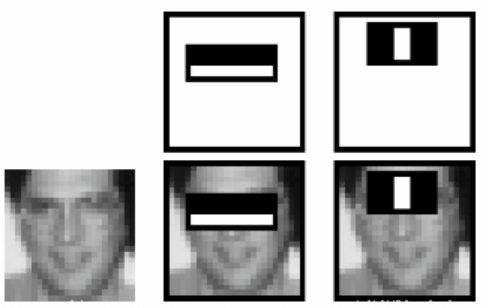
\includegraphics[scale=0.25]{images/kernel2}
\end{figure}
\end{frame}


\begin{frame}{Algorithms Used}
Most of any image is a non-face region. So it is a better idea to have a simple method to check if a window is not a face region then we discard it and never process it to save time. \\~\\

For this they introduced the concept of \textbf{Cascade of Classifiers}. Instead of applying all features on a window, the features are grouped into different stages of classifiers and applied one-by-one. If a window fails at a stage, it won't continue to the remaining feature stages. The window which passes all stages is considered a face region.
\end{frame}



\begin{frame}{Algorithms Used}
\textbf{How we interface this in OpenCV:} \\
\tab OpenCV comes with a trainer as well as detector. If you want to train your own classifier for any specific object like a Pagani Zonda or Mido Khalaf for example. you can use OpenCV to create one. \\~\\

Speaking of the detector, OpenCV already contains many pre-trained classifiers for face, eyes, smiles, ...etc each in an xml file. \\
\end{frame}


\begin{frame}{Algorithms Used}
\textbf{The OpenCV Algorithm in a nutshell:} \\
\tab 1- load the xml files for the objects you want to detect. \\
\tab 2- read the image you want to apply the classifier on, or use the video \\
\tab[0.8cm] feed from your webcam. \\
\tab 3- apply the face detector on the gray-scale verion of the image. \\
\tab 4- apply the eye and smile detector inside the rectangle of the
\tab[0.8cm] detected faces. \\
\tab 5- plot rectangles of unique colours on every feature you detect.
\end{frame}


\section{Results and Discussions}
\begin{frame}{Results and Discussions}

\centering
\textbf{Face Detection}

\begin{figure}
\vspace*{0cm}
\hspace*{0cm}
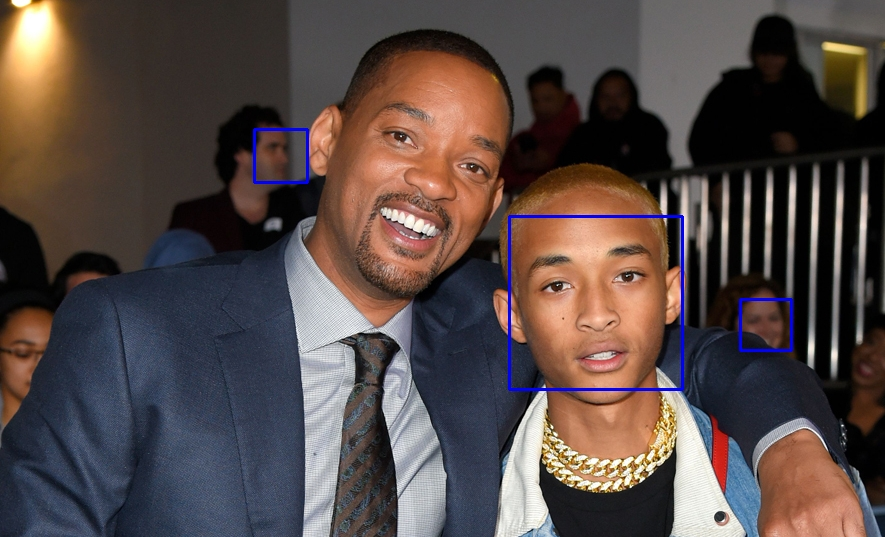
\includegraphics[scale=0.25]{samples/face}
\end{figure}

\small Here we can see that it couldn't detect \textbf{Will's} face because it is a little bit tilted
\end{frame}



\begin{frame}{Results and Discussions}

\centering
\textbf{Face and Eye Detection}

\begin{figure}
\vspace*{0cm}
\hspace*{0cm}
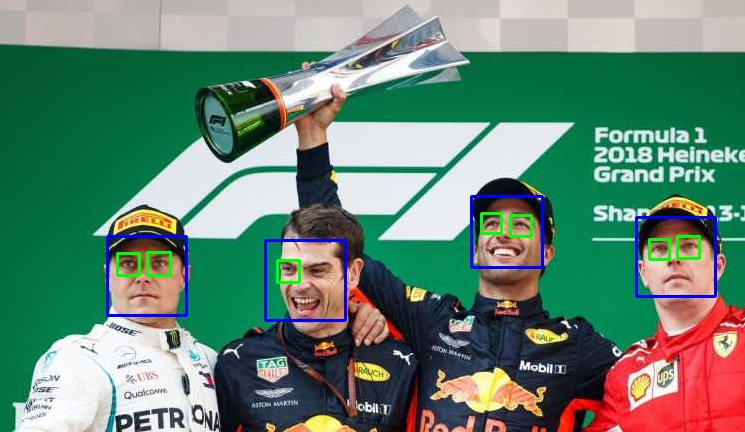
\includegraphics[scale=0.3]{samples/face_eye}
\end{figure}

\small Here, it couldn't detect the RedBull engineer left eye because it is closed.
\end{frame}



\begin{frame}{Results and Discussions}

\centering
\textbf{Face and Smile Detection}

\begin{figure}
\vspace*{0cm}
\hspace*{0cm}
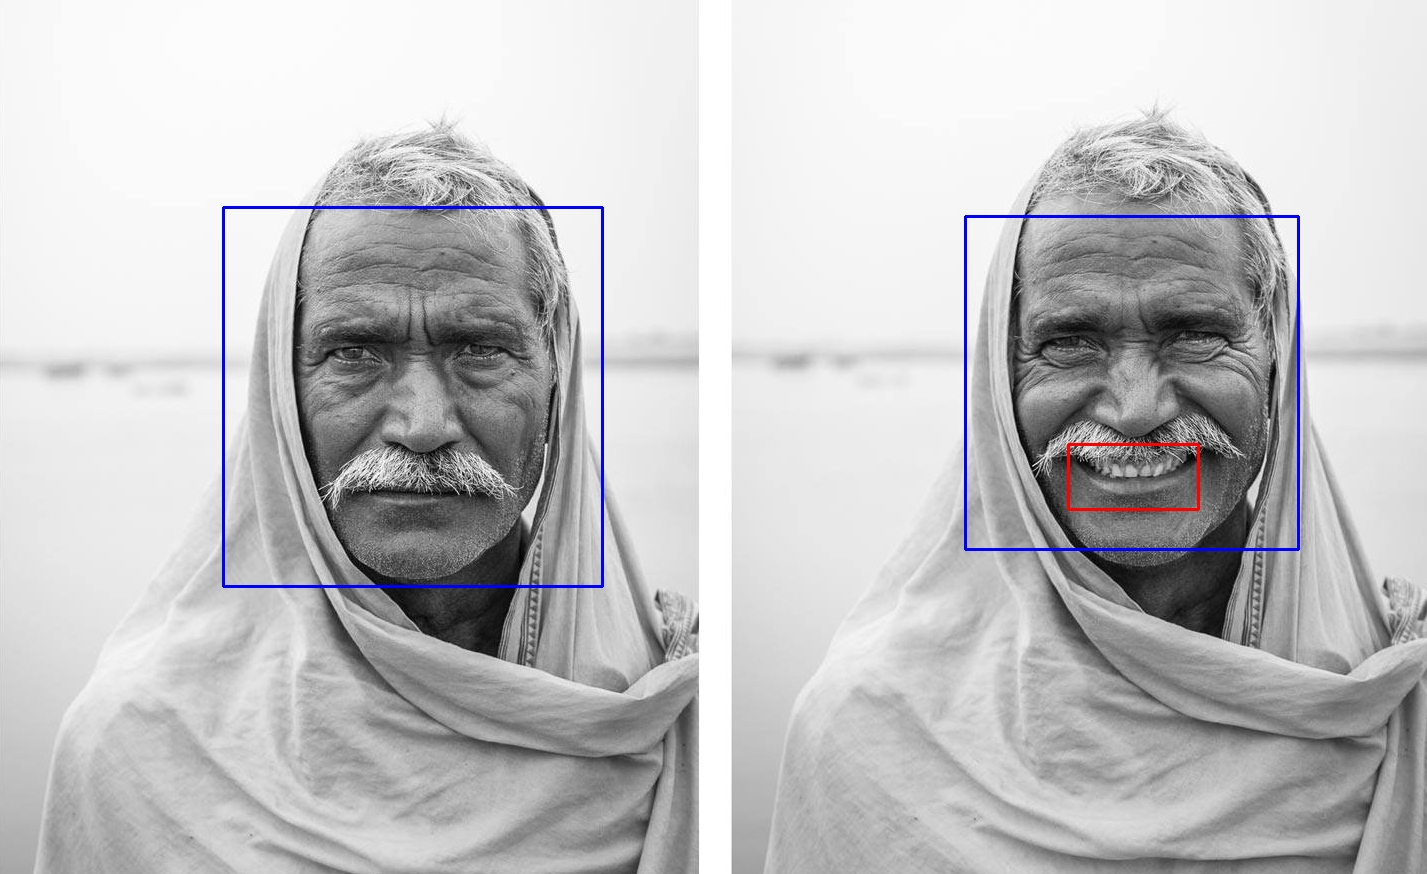
\includegraphics[scale=0.15]{samples/face_smile}
\end{figure}

\small It is flawless in detecting that smile because it is very obvious.
\end{frame}



\begin{frame}{Results and Discussions}

\centering
\textbf{Face and Eye Detection from a Video}

\begin{figure}
\vspace*{0cm}
\hspace*{0cm}
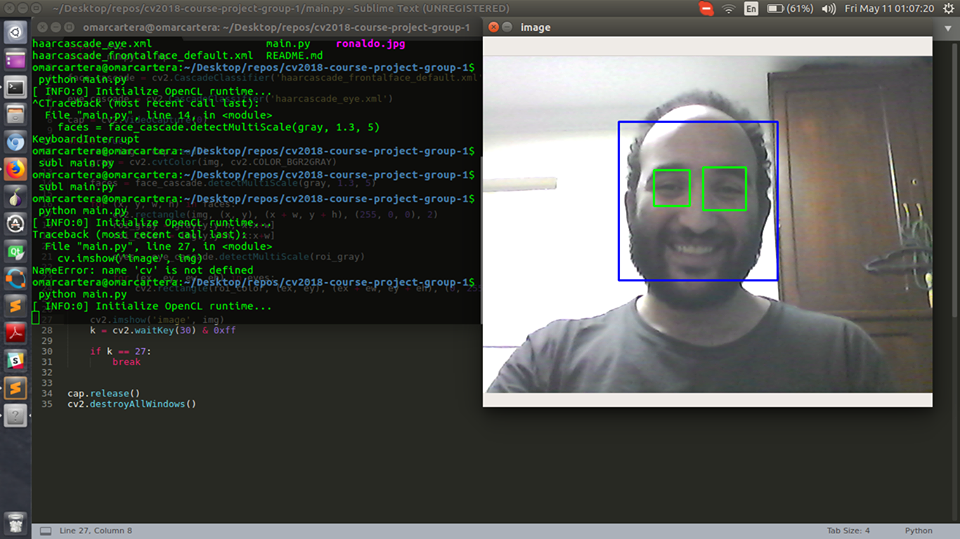
\includegraphics[scale=0.3]{samples/face_eye_video}
\end{figure}
\end{frame}



\section{Limitations}
\begin{frame}{Limitations}
\textbf{The limitations we faced were:} \\
\tab 1- We are using Frontal Face detection, so it will fail to detect side \\ \tab[0.8cm] views. \\
\tab 2- The detector settings don't always work perfectly with each image, \\ \tab[0.8cm] every time you need to tune the \textbf{\textit{detectMultiScale}} \textit{ScaleFactor} \\
\tab[0.8cm] and \textit{MinNeghbors}, and then it works well.
\end{frame}

\vspace*{2.5cm}
\hspace*{3.9cm}
\huge THANKS!

\end{document}
